\documentclass{standalone}
\usepackage{tikz}
\usetikzlibrary{positioning, shapes}

\begin{document}
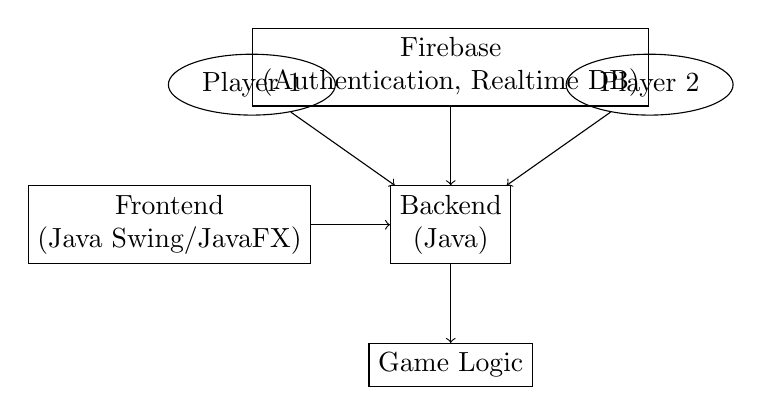
\begin{tikzpicture}[x=2.5cm, y=2.5cm] % Adjust the x and y dimensions as needed
    % Frontend
    \node[draw, rectangle, align=center] (frontend) {Frontend\\(Java Swing/JavaFX)};
    
    % Backend
    \node[draw, rectangle, align=center, right=of frontend] (backend) {Backend\\(Java)};
    
    % Firebase
    \node[draw, rectangle, align=center, above=of backend] (firebase) {Firebase\\(Authentication, Realtime DB)};
    
    % Game Logic
    \node[draw, rectangle, align=center, below=of backend] (game) {Game Logic};
    
    % Players
    \node[draw, ellipse, align=center, above left=of backend.north west] (player1) {Player 1};
    \node[draw, ellipse, align=center, above right=of backend.north east] (player2) {Player 2};
    
    % Arrows
    \draw[->] (frontend) -- (backend);
    \draw[->] (backend) -- (game);
    \draw[->] (firebase) -- (backend);
    \draw[->] (player1) -- (backend);
    \draw[->] (player2) -- (backend);
\end{tikzpicture}
\end{document}
